\documentclass{standalone}
\usepackage{tikz}
\usetikzlibrary{patterns, positioning}
\usepackage[sfdefault]{ClearSans} %% option 'sfdefault' activates Clear Sans as the default text font
\usepackage[T1]{fontenc}

\begin{document}
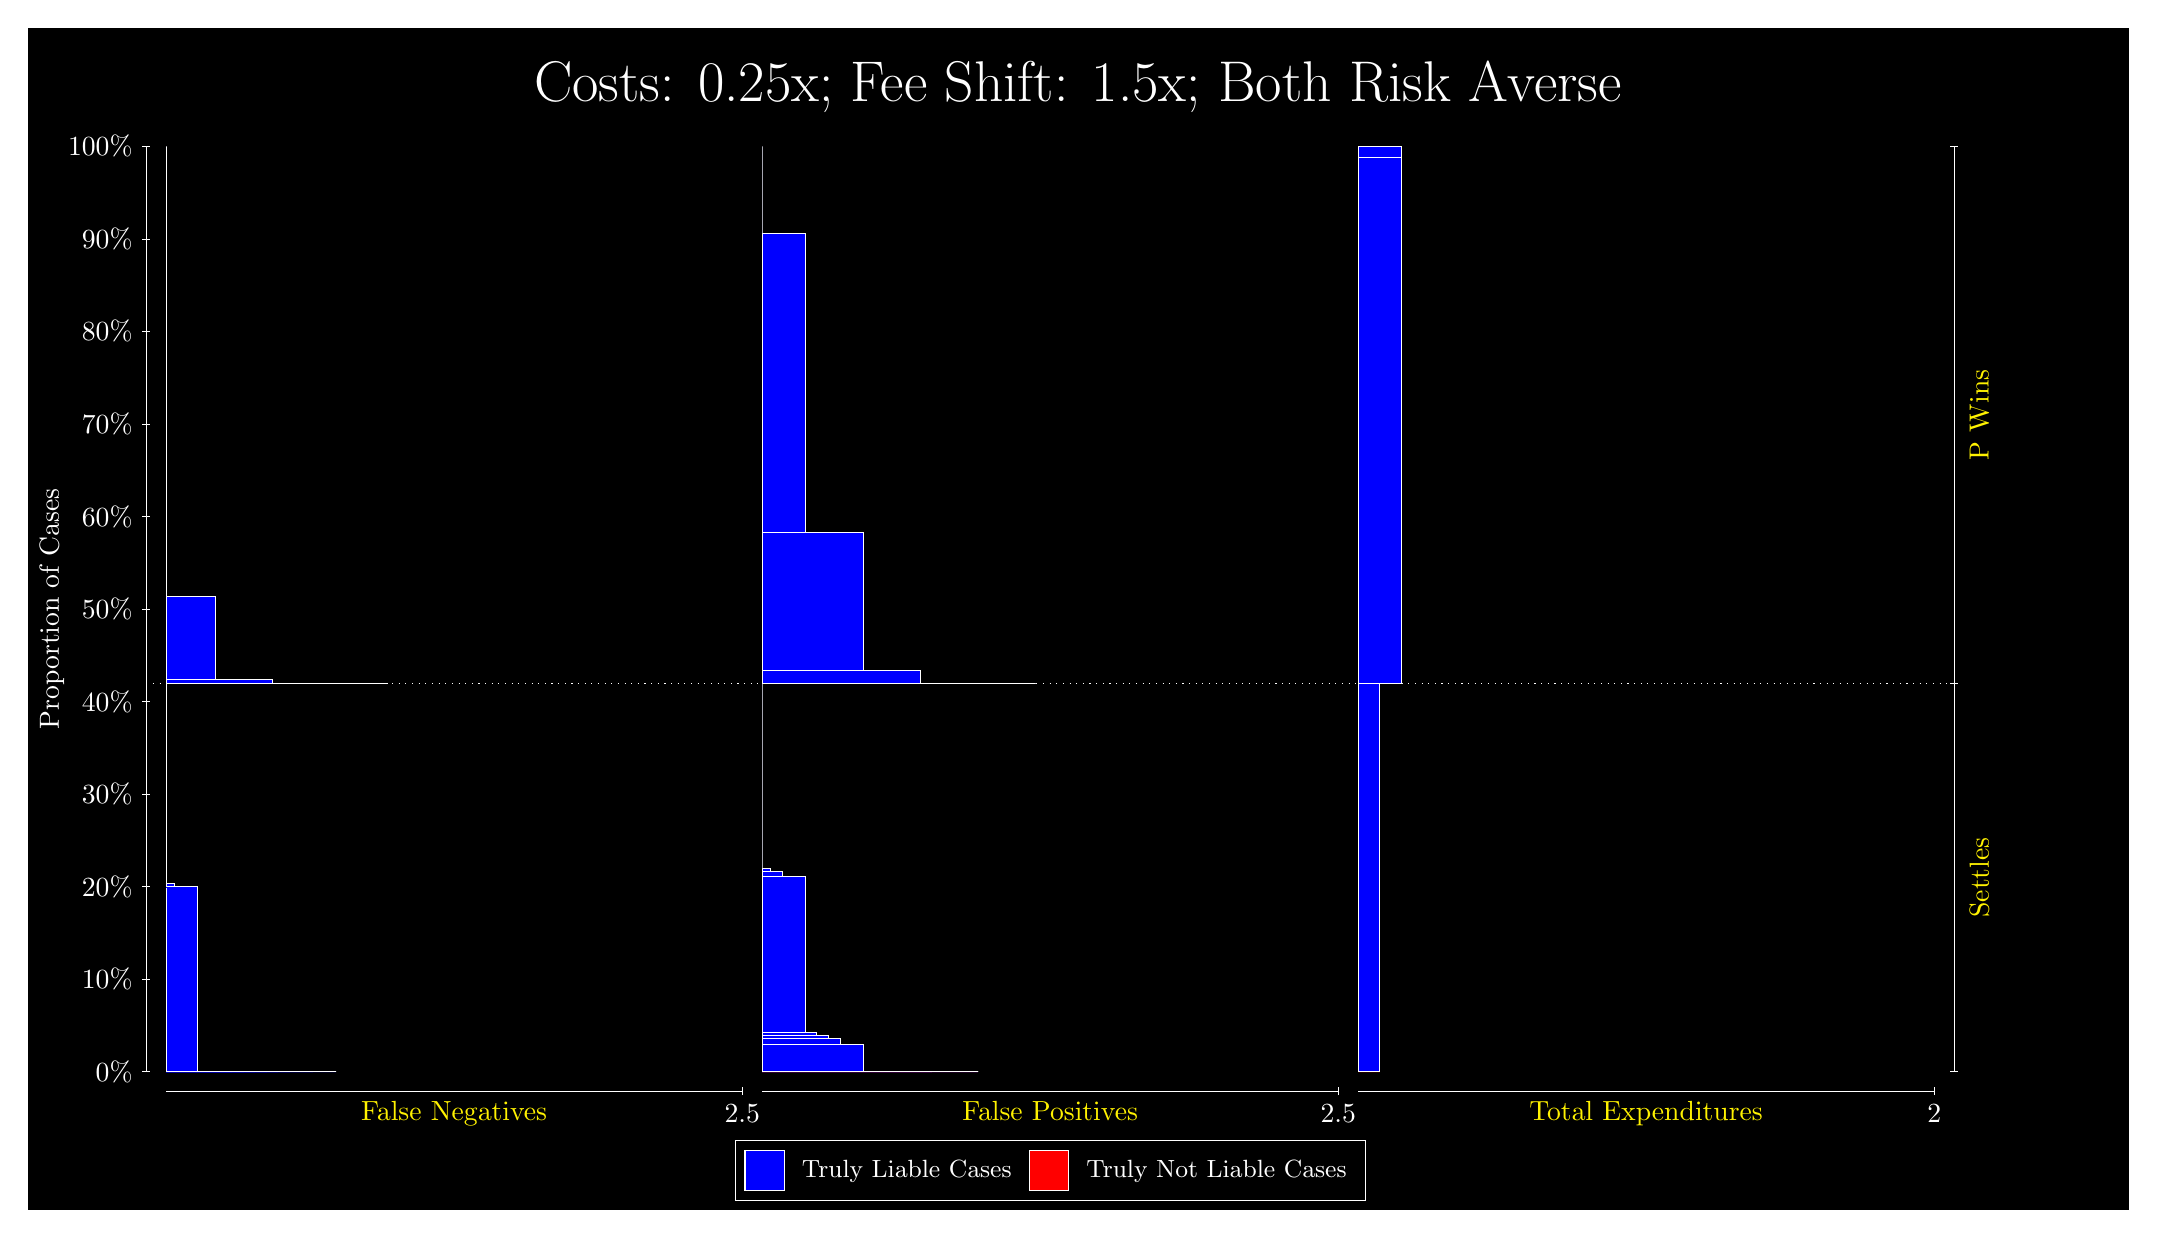
\begin{tikzpicture}
\draw[fill=black] (0,0) rectangle (26.667,15);
\draw[text=white] (0,13.5) rectangle (26.667,15) node[midway] {\huge Costs: 0.25x; Fee Shift: 1.5x; Both Risk Averse};
\draw[white, very thin] (1.5,1.75) -- (1.5,13.5);
\node[rotate=90, text=white, anchor=center] at (0.3, 7.625) {Proportion of Cases};
\draw[white, very thin] (1.45,1.75) -- (1.55,1.75);
\node[text=white, anchor=east] at (1.45, 1.75) {0\%};
\draw[white, very thin] (1.45,2.925) -- (1.55,2.925);
\node[text=white, anchor=east] at (1.45, 2.925) {10\%};
\draw[white, very thin] (1.45,4.1) -- (1.55,4.1);
\node[text=white, anchor=east] at (1.45, 4.1) {20\%};
\draw[white, very thin] (1.45,5.275) -- (1.55,5.275);
\node[text=white, anchor=east] at (1.45, 5.275) {30\%};
\draw[white, very thin] (1.45,6.45) -- (1.55,6.45);
\node[text=white, anchor=east] at (1.45, 6.45) {40\%};
\draw[white, very thin] (1.45,7.625) -- (1.55,7.625);
\node[text=white, anchor=east] at (1.45, 7.625) {50\%};
\draw[white, very thin] (1.45,8.8) -- (1.55,8.8);
\node[text=white, anchor=east] at (1.45, 8.8) {60\%};
\draw[white, very thin] (1.45,9.975) -- (1.55,9.975);
\node[text=white, anchor=east] at (1.45, 9.975) {70\%};
\draw[white, very thin] (1.45,11.15) -- (1.55,11.15);
\node[text=white, anchor=east] at (1.45, 11.15) {80\%};
\draw[white, very thin] (1.45,12.325) -- (1.55,12.325);
\node[text=white, anchor=east] at (1.45, 12.325) {90\%};
\draw[white, very thin] (1.45,13.5) -- (1.55,13.5);
\node[text=white, anchor=east] at (1.45, 13.5) {100\%};

\draw[white, very thin] (24.457,1.75) -- (24.457,13.5);
\draw[white, very thin] (24.407,1.75) -- (24.507,1.75);
\node[anchor=west] at (24.407, 1.75) {};
\draw[white, very thin] (24.407,6.6794) -- (24.507,6.6794);
\node[anchor=west] at (24.407, 6.6794) {};
\draw[white, very thin] (24.407,13.5) -- (24.507,13.5);
\node[anchor=west] at (24.407, 13.5) {};

\draw[white, very thin, fill=blue] (1.75,1.75) rectangle (3.9091,1.75);
\draw[white, very thin, fill=blue] (1.75,1.75) rectangle (3.6163,1.75);
\draw[white, very thin, fill=blue] (1.75,1.75) rectangle (3.3236,1.75);
\draw[white, very thin, fill=blue] (1.75,1.75) rectangle (3.1772,1.75);
\draw[white, very thin, fill=blue] (1.75,1.75) rectangle (3.0308,1.75);
\draw[white, very thin, fill=blue] (1.75,1.75) rectangle (2.8844,1.75);
\draw[white, very thin, fill=blue] (1.75,1.75) rectangle (2.738,1.75);
\draw[white, very thin, fill=blue] (1.75,1.75) rectangle (2.5917,1.7501);
\draw[white, very thin, fill=blue] (1.75,1.7501) rectangle (2.4453,1.7506);
\draw[white, very thin, fill=blue] (1.75,1.7506) rectangle (2.2989,1.7506);
\draw[white, very thin, fill=blue] (1.75,1.7506) rectangle (2.1525,4.0971);
\draw[white, very thin, fill=blue] (1.75,4.0971) rectangle (2.0062,4.0983);
\draw[white, very thin, fill=blue] (1.75,4.0983) rectangle (1.8598,4.142);
\draw[white, very thin, fill=red] (1.75,4.142) rectangle (1.75,4.142);
\draw[white, very thin, fill=blue] (1.75,4.142) rectangle (1.75,6.6794);
\draw[white, very thin, fill=blue] (1.75,6.6794) rectangle (4.5678,6.6794);
\draw[white, very thin, fill=blue] (1.75,6.6794) rectangle (3.8359,6.6796);
\draw[white, very thin, fill=blue] (1.75,6.6796) rectangle (3.104,6.7314);
\draw[white, very thin, fill=blue] (1.75,6.7314) rectangle (2.3721,7.789);
\draw[white, very thin, fill=red] (1.75,7.789) rectangle (1.75,7.789);
\draw[white, very thin, fill=blue] (1.75,7.789) rectangle (1.75,13.5);
\draw[white, very thin, fill=red] (9.3189,1.75) rectangle (12.063,1.75);
\draw[white, very thin, fill=blue] (9.3189,1.75) rectangle (12.063,1.75);
\draw[white, very thin, fill=red] (9.3189,1.75) rectangle (11.478,1.75);
\draw[white, very thin, fill=blue] (9.3189,1.75) rectangle (11.478,1.75);
\draw[white, very thin, fill=blue] (9.3189,1.75) rectangle (11.332,1.7519);
\draw[white, very thin, fill=red] (9.3189,1.7519) rectangle (11.185,1.7519);
\draw[white, very thin, fill=blue] (9.3189,1.7519) rectangle (11.185,1.7519);
\draw[white, very thin, fill=red] (9.3189,1.7519) rectangle (10.892,1.7519);
\draw[white, very thin, fill=blue] (9.3189,1.7519) rectangle (10.892,1.7522);
\draw[white, very thin, fill=blue] (9.3189,1.7522) rectangle (10.746,1.7533);
\draw[white, very thin, fill=red] (9.3189,1.7533) rectangle (10.6,1.7533);
\draw[white, very thin, fill=blue] (9.3189,1.7533) rectangle (10.6,2.1001);
\draw[white, very thin, fill=blue] (9.3189,2.1001) rectangle (10.453,2.1003);
\draw[white, very thin, fill=red] (9.3189,2.1003) rectangle (10.307,2.1003);
\draw[white, very thin, fill=blue] (9.3189,2.1003) rectangle (10.307,2.1687);
\draw[white, very thin, fill=blue] (9.3189,2.1687) rectangle (10.161,2.2166);
\draw[white, very thin, fill=blue] (9.3189,2.2166) rectangle (10.014,2.243);
\draw[white, very thin, fill=blue] (9.3189,2.243) rectangle (9.8678,4.2286);
\draw[white, very thin, fill=blue] (9.3189,4.2286) rectangle (9.7214,4.2288);
\draw[white, very thin, fill=blue] (9.3189,4.2288) rectangle (9.575,4.2874);
\draw[white, very thin, fill=blue] (9.3189,4.2874) rectangle (9.4287,4.3311);
\draw[white, very thin, fill=blue] (9.3189,4.3311) rectangle (9.3189,6.6794);
\draw[white, very thin, fill=red] (9.3189,6.6794) rectangle (12.795,6.6794);
\draw[white, very thin, fill=blue] (9.3189,6.6794) rectangle (12.795,6.6794);
\draw[white, very thin, fill=red] (9.3189,6.6794) rectangle (12.063,6.6794);
\draw[white, very thin, fill=blue] (9.3189,6.6794) rectangle (12.063,6.6817);
\draw[white, very thin, fill=red] (9.3189,6.6817) rectangle (11.332,6.6817);
\draw[white, very thin, fill=blue] (9.3189,6.6817) rectangle (11.332,6.8439);
\draw[white, very thin, fill=red] (9.3189,6.8439) rectangle (10.6,6.8439);
\draw[white, very thin, fill=blue] (9.3189,6.8439) rectangle (10.6,8.6013);
\draw[white, very thin, fill=red] (9.3189,8.6013) rectangle (9.8678,8.6013);
\draw[white, very thin, fill=blue] (9.3189,8.6013) rectangle (9.8678,12.39);
\draw[white, very thin, fill=blue] (9.3189,12.39) rectangle (9.3189,13.5);
\draw[white, very thin, fill=red] (16.888,1.75) rectangle (17.162,1.75);
\draw[white, very thin, fill=blue] (16.888,1.75) rectangle (17.162,6.6794);
\draw[white, very thin, fill=red] (16.888,6.6794) rectangle (17.437,6.6794);
\draw[white, very thin, fill=blue] (16.888,6.6794) rectangle (17.437,13.366);
\draw[white, very thin, fill=red] (16.888,13.366) rectangle (17.437,13.366);
\draw[white, very thin, fill=blue] (16.888,13.366) rectangle (17.437,13.5);
\draw[white, dotted] (1.5,6.6794) -- (24.457,6.6794);
\draw[white, very thin] (1.75,1.5) -- (9.0689,1.5);
\node[text=yellow, anchor=north] at (5.4094, 1.5) {False Negatives};
\draw[white, very thin] (9.0689,1.45) -- (9.0689,1.55);
\node[text=white, anchor=north] at (9.0689, 1.45) {2.5};

\draw[white, very thin] (9.3189,1.5) -- (16.638,1.5);
\node[text=yellow, anchor=north] at (12.978, 1.5) {False Positives};
\draw[white, very thin] (16.638,1.45) -- (16.638,1.55);
\node[text=white, anchor=north] at (16.638, 1.45) {2.5};

\draw[white, very thin] (16.888,1.5) -- (24.207,1.5);
\node[text=yellow, anchor=north] at (20.547, 1.5) {Total Expenditures};
\draw[white, very thin] (24.207,1.45) -- (24.207,1.55);
\node[text=white, anchor=north] at (24.207, 1.45) {2};

\node[text=yellow, centered, rotate=90] at (24.777, 4.2147) {Settles};
\node[text=yellow, centered, rotate=90] at (24.777, 10.09) {P Wins};

\draw (12.978300999999998,1.5) node[draw=none] (baseCoordinate) {};
\begin{scope}[align=center]
        \matrix[scale=0.5, draw=white, below=0.5cm of baseCoordinate, nodes={draw}, column sep=0.1cm]{
            \node[rectangle, draw, minimum width=0.5cm, minimum height=0.5cm, fill=blue] {}; &
            \node[draw=none, font=\small, text=white] (B) {Truly Liable Cases}; &
            \node[rectangle, draw, minimum width=0.5cm, minimum height=0.5cm, fill=red] {}; &
            \node[draw=none, font=\small, text=white] (B) {Truly Not Liable Cases}; \\
            };
\end{scope}

\end{tikzpicture}
\end{document}